\documentclass{article}
\usepackage[a4paper, total={6.5in, 10in}]{geometry}
\usepackage[utf8]{inputenc}
\usepackage[T1]{fontenc}
\usepackage{polski}
\usepackage{amsfonts}
\usepackage{graphicx}
\usepackage{enumitem}
\usepackage{pgfgantt}
\usepackage{pgfplots}
\pgfplotsset{width=10cm,compat=1.9}

\usepgfplotslibrary{fillbetween}
\usetikzlibrary{patterns}

\title{WSYZ kolokwium 2, zestaw 2 - rozwiązania}
\author{Jakub Ostrzołek}

\begin{document}
\maketitle

\section*{Zadanie 1.}

\section*{Zadanie 2.}
\subsection*{$k < 2$}

brak rozwiązania

\subsection*{$k \in \{2, 3\}:$}

Tylko jedna para pracowników może pracować na raz.
Pracownicy wykonają swoje zadanie sekwencyjnie.

$$T_{min} = \sum_{m \in M} p_m = 82$$

\subsection*{$k \in \{4, 5\}:$}

\begin{ganttchart}[
        expand chart=\textwidth
    ]{1}{45}
    \gantttitlelist{1,...,45}{1} \\
    \ganttbar{P1}{1}{0}
    \ganttbar[inline]{M1}{1}{13}
    \ganttbar[inline]{M4}{14}{28}
    \ganttbar[inline]{M8}{29}{38}
    \ganttbar[inline]{M7}{39}{42}
    \\
    \ganttbar{P2}{1}{0}
    \ganttbar[inline]{M2}{1}{8}
    \ganttbar[inline]{M3}{14}{22}
    \ganttbar[inline]{M6}{23}{25}
    \ganttbar[inline]{M5}{26}{45}
\end{ganttchart}

$$T_{min} = 45$$

\subsection*{$k \ge 6:$}

W tym przypadku wszystkie nie-krytyczne zadania zdążą się wykonać
podczas gdy jedna para pracowników będzie wykonywała zadania ze
ścieżki krytycznej. Dlatego $T_{min}$ to będzie długość ścieżki
krytycznej.

$$T_{min} = 38$$

\section*{Zadanie 3}

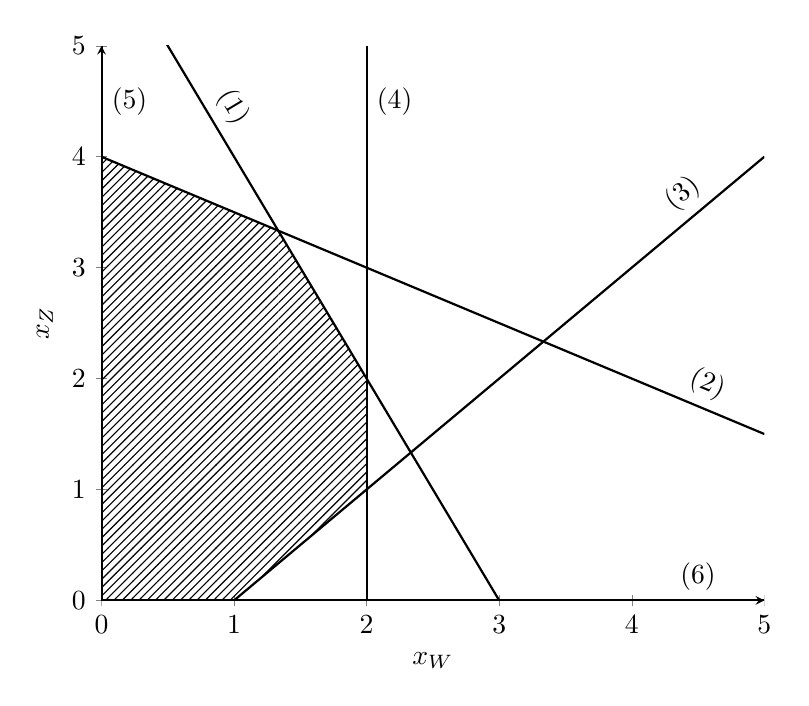
\begin{tikzpicture}
    \begin{axis}[
        axis lines=left,
        xlabel=$x_W$,
        ylabel=$x_Z$,
        domain=0:5,
        ymin=0,
        ymax=5,
        restrict y to domain=-1:6
    ]
        \addplot[color=black, thick, name path=1]{6 - 2*x} node[pos=0.25, sloped, above] {(1)};
        \addplot[color=black, thick, name path=2]{4 - 1/2*x} node[pos=0.9, sloped, above] {(2)};
        \addplot[color=black, thick, name path=3]{x - 1} node[pos=0.9, sloped, above] {(3)};
        \addplot[color=black, thick, name path=4] coordinates {
            (2, \pgfkeysvalueof{/pgfplots/ymin})
            (2, \pgfkeysvalueof{/pgfplots/ymax})} node[pos=0.9, right] {(4)};
        \addplot[color=black, thick, name path=yaxis] coordinates {
            (0, \pgfkeysvalueof{/pgfplots/ymin})
            (0, \pgfkeysvalueof{/pgfplots/ymax})} node[pos=0.9, right] {(5)};
        \addplot[color=black, thick, name path=xaxis]{0} node[pos=0.9, sloped, above] {(6)};;
        \addplot[gray, pattern=north east lines] fill between[of=2 and 3, soft clip={domain=0:4/3}];
        \addplot[gray, pattern=north east lines] fill between[of=1 and 3, soft clip={domain=4/3:2}];
    \end{axis}
\end{tikzpicture}

\section*{Zadanie 6}
$$\min{v_0} = 6v_1 + 8v_2 + v_3 + 2v_4$$
$$2v_1 + v_2 + v_3 + v_4 \ge 20$$
$$v_1 + 2v_2 - v_3 \ge 30$$
$$v_1, v_2, v_3, v_4 \ge 0$$

\end{document}